\documentclass[11pt]{article}
\usepackage[utf8]{inputenc}
\usepackage{graphicx}
\usepackage{caption}
\usepackage{subcaption}
\usepackage{amsmath}
\usepackage{float}


\title{
	{Computer Vision 1 - Assignment 3 \\
	Harris Corner Detector and Optical Flow}
}
\author{
Selene Baez Santamaria (10985417) - Andrea Jemmett (11162929)}
\date{\today}

\begin{document}

\maketitle

\section{Harris Corner Detector}
% Question: "Demo function"
To implement the Harris Corner Detector we decided to use the function we
implemented on previous assignments. This way we can exploit the benefits of
kernel separability and improve performance. Thus, we created horizontal and
vertical Gaussian kernels, and applied a Gaussian first order derivative kernel to the image, read in a gray scale format. The image gradients are shown in Figure
\ref{fig:partialDerivatives_pingpong} and \ref{fig:partialDerivatives_person}.

\begin{figure}[H] \centering
	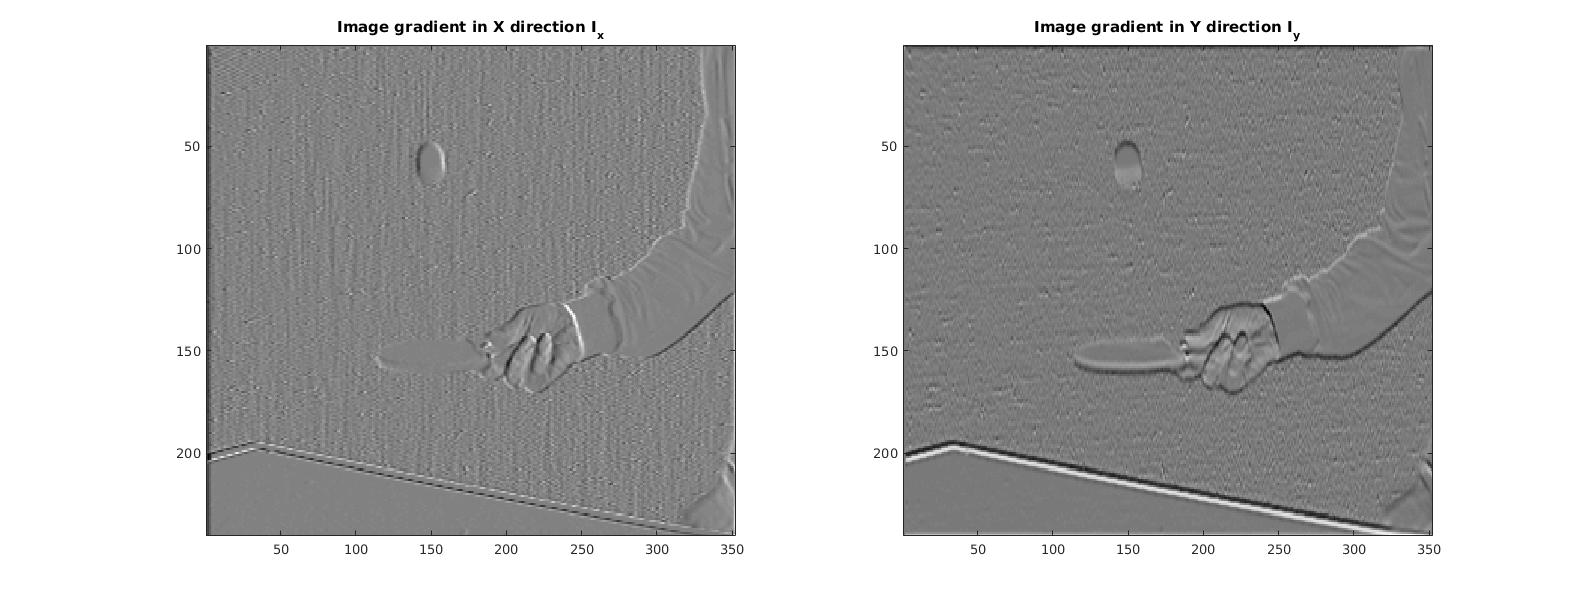
\includegraphics[width=1\textwidth]{imgs/derivatives_pingpong.jpg}
	\caption{Image gradients for first Ping Pong image}
	\label{fig:partialDerivatives_pingpong}
\end{figure}

\begin{figure}[H] \centering
	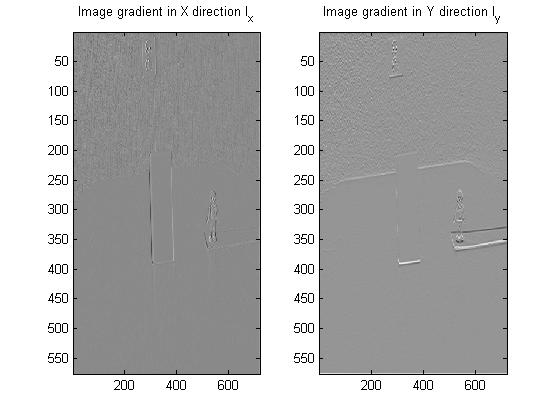
\includegraphics[width=1\textwidth]{imgs/derivatives_person.jpg}
	\caption{Image gradients for first Toy Person image}
	\label{fig:partialDerivatives_person}
\end{figure}

Then, we created the $Q$ matrix, first by squaring the gradients (i.e.
$I_{x}^2$ and $I_{y}^2$) and multiplying them with each other (i.e. $I_x
I_y$), and then by convolving the resulting with a Gaussian kernel. With these
components we were able to compute $H$ using Equation $12$ shown in the
assignment instructions. We also scale the corner metric by a $\frac{1000}{
max(H)}$ factor; this to avoid using a threshold value of the magnitude of
$e^{-6}$. A visualization for the scaled surfaces are shown in
Figure \ref{fig:surface_pingpong} and \ref{fig:surface_person}.

\begin{figure}[H] \centering
	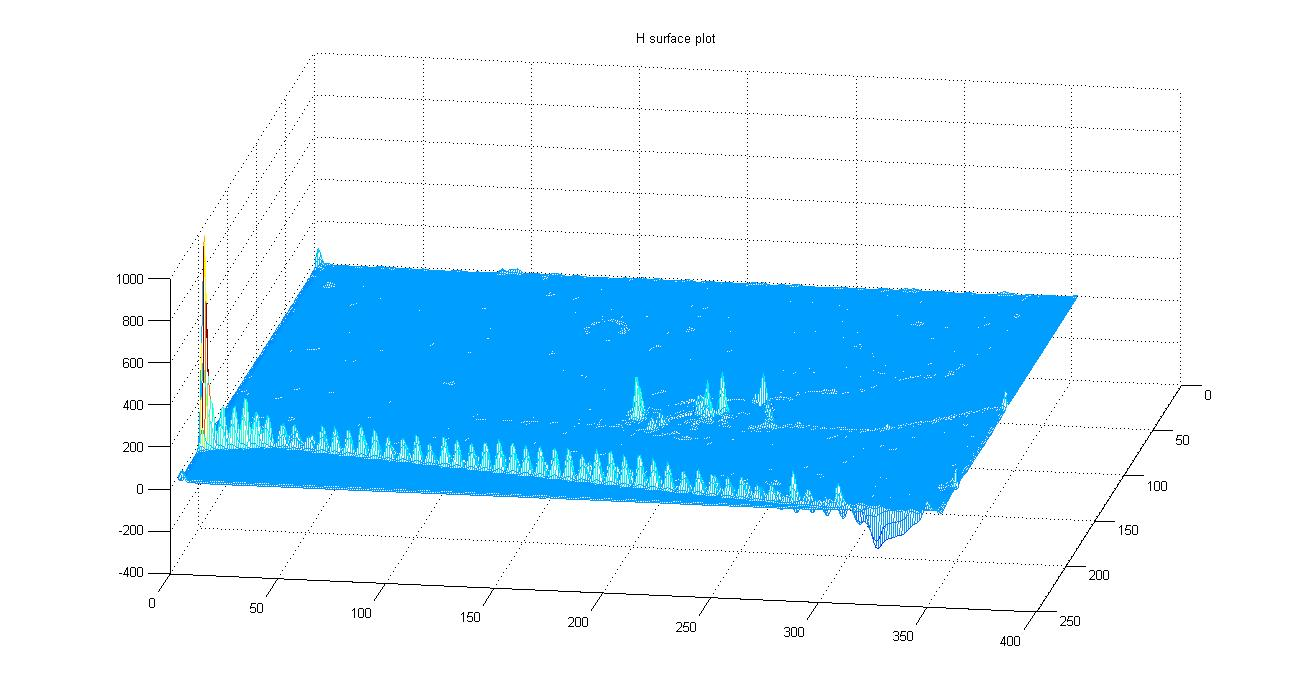
\includegraphics[width=.8\textwidth]{imgs/surface_pingpong.jpg}
	\caption{$H$ surface for first Ping Pong image. Local maxima are
		observed along the ping pong table, and the hand.}
	\label{fig:surface_pingpong}
\end{figure}

\begin{figure}[H] \centering
	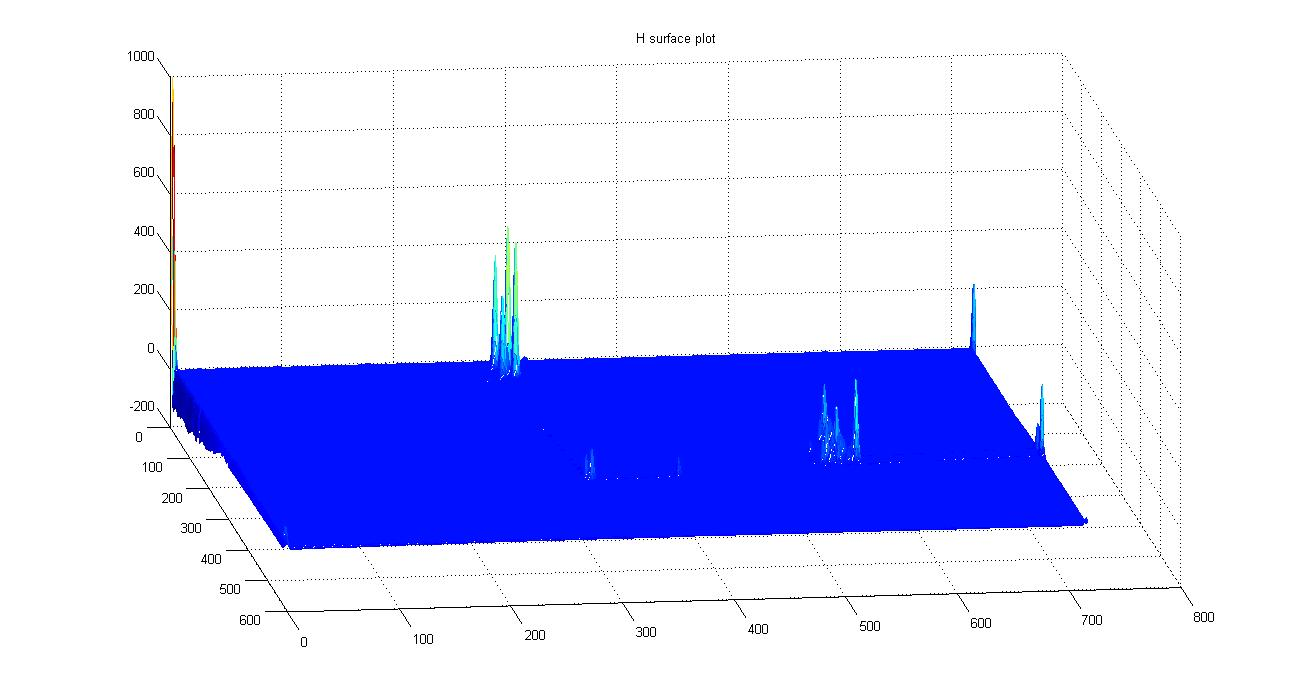
\includegraphics[width=.8\textwidth]{imgs/surface_person.jpg}
	\caption{$H$ surface for first Toy Person image. Local maxima are
		observed on the power outlet and on the toy person.}
	\label{fig:surface_person}
\end{figure}

Finally, to choose the corner points we considered two conditions:
\begin{enumerate} 
	\item A corner point must be a local maximum. To check for
		this we need to compare its value with all its neighbors' within
		a given window.
	\item A corner point must have a higher $H$
		value than a given threshold.
\end{enumerate}

To create an accurate corner detector we need to tune the parameters. We know
that $\sigma$ controls the smoothness of surface $H$. When $\sigma \gg 1$, the
smoothing is so hard that the local maxima are identified in the flat regions
like the center of the pingpong ball in Figure \ref{fig:surface_pingpong_s10}.  
$\sigma \ll 1$ introduces noise by detecting corner points in the background. The
window size determines the closeness at which points may be, therefore a larger
window prevents them from clustering and reduces the final amount of points.
Finally, the threshold regulates the pressure for candidate points to become
corner points. Thus, a higher threshold reduces the final number of points.

\begin{figure}[H] \centering
	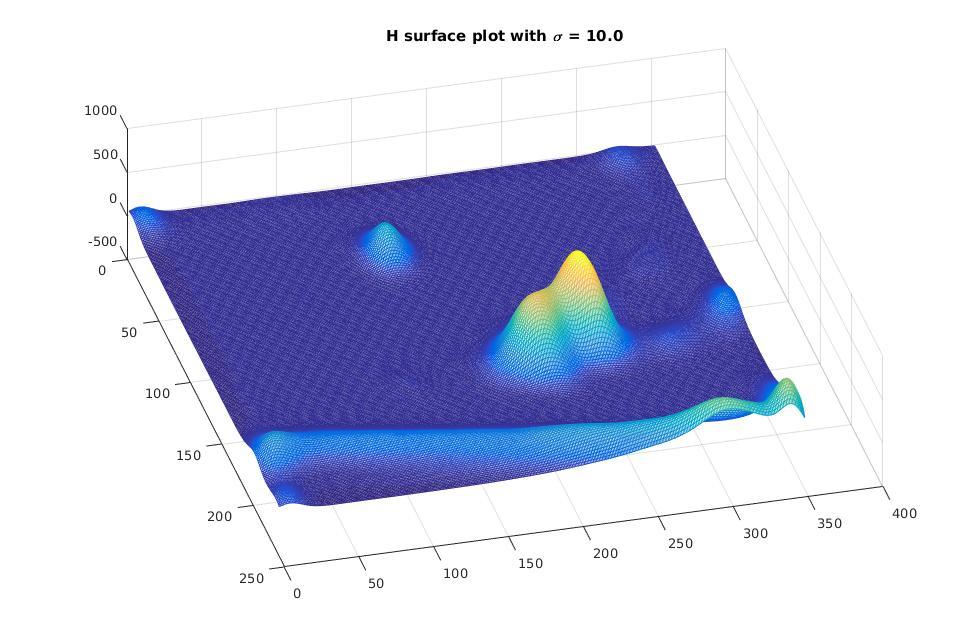
\includegraphics[width=.8\textwidth]{imgs/surface_pingpong_s10.jpg}
	\caption{$H$ surface for first Ping Pong image with $\sigma$ set to $10$. It is
	easy to see that the entire ball could be identified as a feature.}
	\label{fig:surface_pingpong_s10}
\end{figure}

After tuning, the chosen values for the final detector are:

\begin{center}
	\begin{tabular}{| c | c |}
		\hline
		\textbf{kernel length} & 11   \\ \hline
		\textbf{$\sigma$}      & 1.5  \\ \hline
		\textbf{window size}   & 11   \\ \hline
		\textbf{threshold}     & 10   \\
		\hline
	\end{tabular}
\end{center}

To validate our detector we compared it with the Matlab \emph{corner} function. In
order to have a fair comparison, we make it so that the built in function
returns the same number of points as our detector (by passing the number of
features found by our implementation as a second parameter) and qualitatively
compare them by visually plotting the corner points.
 
\begin{figure}[H] \centering
	\begin{subfigure}{.5\textwidth} \centering
		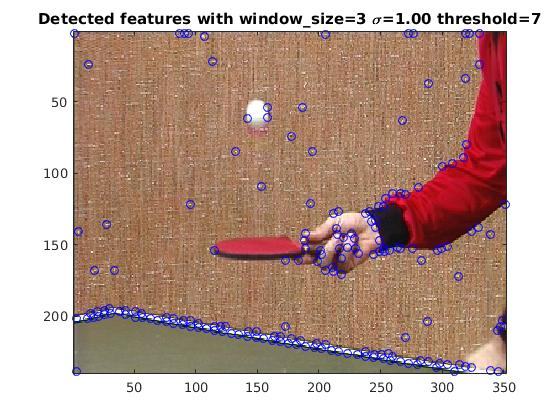
\includegraphics[width=1\textwidth]{imgs/ourCorners_pingpong.jpg}
		\caption{Our implementation of Harris Corner Detector.}
		\label{fig:ourCorners_pingpong}
	\end{subfigure}%
	\begin{subfigure}{.5\textwidth} \centering
		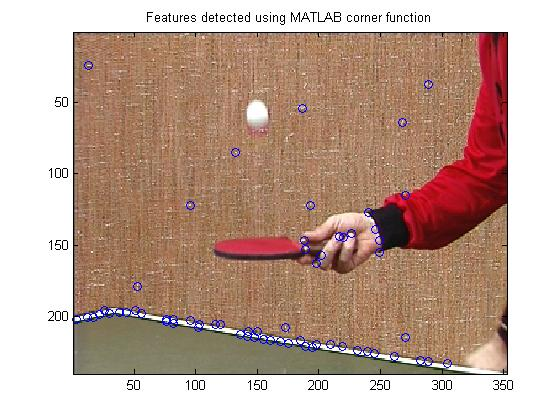
\includegraphics[width=1\textwidth]{imgs/matlabCorners_pingpong.jpg}
		\caption{Matlab's built in Corner function.}
		\label{fig:matlabCorners_pingpong}
	\end{subfigure}
	\caption{Corner points in first Ping Pong image}
	\label{fig:corners_pingpong}
\end{figure}

\begin{figure}[H]
	\centering
	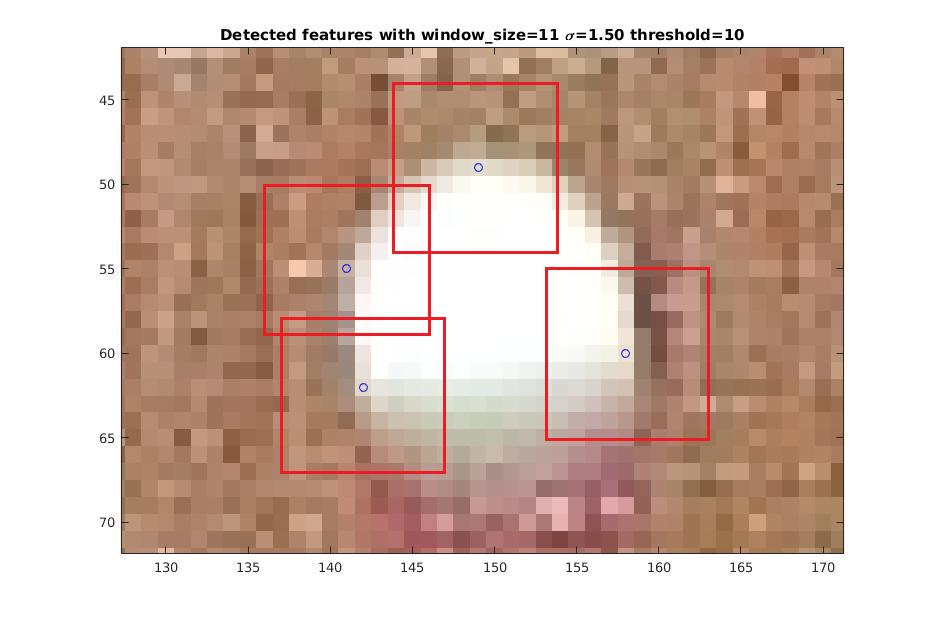
\includegraphics[width=.8\textwidth]{imgs/ball_feature_corners.jpg}
	\caption{Zoomed region around the Ping Pong ball. In blue are the detected
	features and in red are the corresponding windows. It's easy to see their
	corner-like shape.}
	\label{fig:ball_corners}
\end{figure}

In case of the Ping Pong image our feature implementation detects $n_{corners} =
63$ (given the aforementioned parameters) and the results are visible in Figure
\ref{fig:ourCorners_pingpong}. On one hand, our detector is able to detect
points around the ball (Figure \ref{fig:ball_corners}) and along the sleeve. On
the other hand, the Matlab function introduces noisy points in the background
and fails to detect the racket, as shown in Figure
\ref{fig:matlabCorners_pingpong}.

\begin{figure}[H] \centering
	\begin{subfigure}{.5\textwidth} \centering
		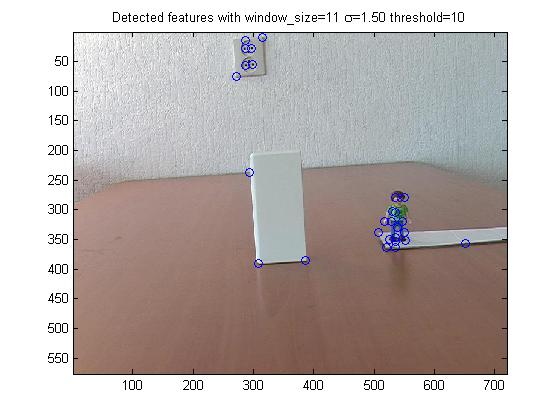
\includegraphics[width=1\textwidth]{imgs/ourCorners_person.jpg}
		\caption{Our implementation of Harris Corner Detector.}
		\label{fig:ourCorners_person}
	\end{subfigure}%
	\begin{subfigure}{.5\textwidth}	\centering
		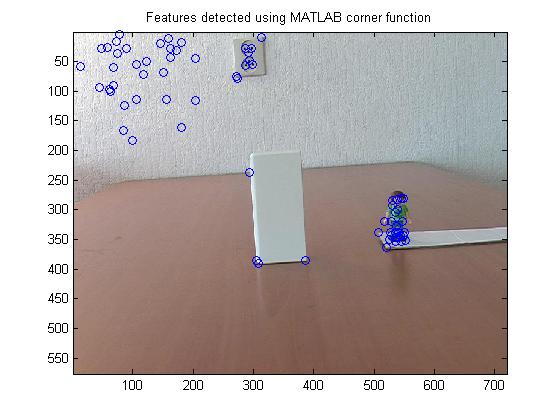
\includegraphics[width=1\textwidth]{imgs/matlabCorners_person.jpg}
		\caption{Matlab's built in Corner function.}
		\label{fig:matlabCorners_person}
	\end{subfigure}
	\caption{Corner points in first Toy person image}
	\label{fig:corners_person}
\end{figure}

In case of the Toy Person image, with the given parameters, out implementation
detects $n_{corners} = 27$. Our detector finds more corner points in the frame
of the power outlet and detects three of the four edges of the white central
box, as show in Figure \ref{fig:ourCorners_person}. The Matlab function
instead focuses more on the toy and its detected features seem more uniquely
identifiable in the image.

\section{Lucas-Kanade Algorithm for Optical Flow}
In order to implement the Lucas Kanade method for Optical Flow estimation, we started by
computing the gradient of the images along the $X$ and $Y$ directions using a Gaussian
kernel as stated in the previous section. This time the tuned parameters are as follows: 

\begin{center}
	\begin{tabular}{| c | c |}
		\hline
		\textbf{kernel length} & 5   \\ \hline
		\textbf{$\sigma$}      & 1  \\ 
		\hline
	\end{tabular}
\end{center}

% To get the full partial $x-y$ derivatives, we added the corresponding gradients from image in $t_1$ and $t_2$.
% NOT SURE WHY? ASSIGNMENT SAYS IT?S ONLY DERIVATIVE EVALUATED AT CURRENT TIME.
To obtain the $t$ gradient we simply convolve the images with a uniform kernel
of value $0.5$ and then we subtract $t_2$ from $t_1$.

To exploit the assumption made by Lucas-Kanade we divide the image into
non-overlapping regions. The region size is a parameter that can be tuned, and
in this case is set as $region\_size= 15$ as recommended by the assignment instructions. Then, for each region we solved the
system of equations to find an estimation of the $x-y$ velocities of the
pixel $p$ placed at the center of the region.

For convenience we created a helper function $solve-region$ to solve the system
of equations for a single region. This function takes the region's center
coordinates $p_x$ and $p_y$, the window's size and the image derivatives in $X$,
$Y$ and $t$ direction and constructs $A = [I_x I_y)]$ and $b = -I_t$ using the
image gradients at the specified region. Those are then used to solve the
following system:
$$V = (A^TA)^{-1}A^Tb$$
which yelds $V = <u, v>$, the displacement matrix for $p$, the region's center.

The final step is to plot the velocity vectors on top of the image. First, we show the image and $hold on$ the figure, so that then we can plot the velocities with the Matlab $quiver$ function on top of it. The results obtained for the sphere and synth images are shown in Figure \ref{fig:sphere_lucas} and \ref{fig:synth_lucas}.


\begin{figure}[H] \centering
	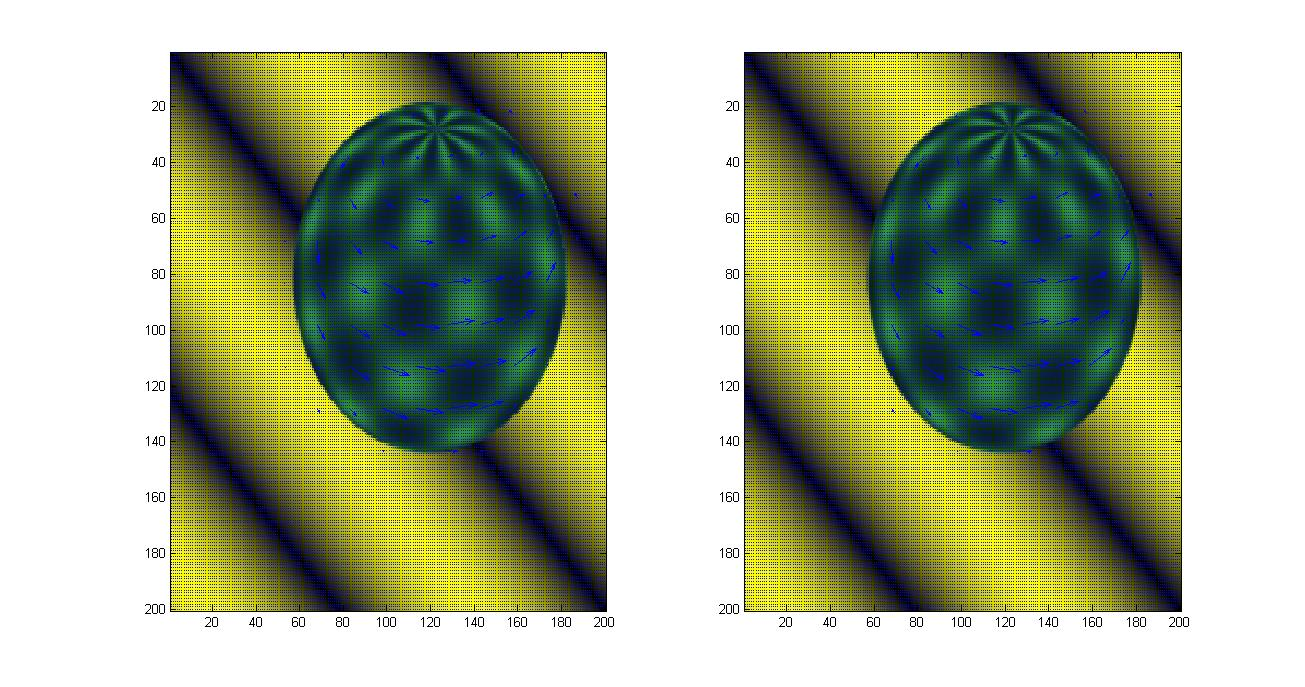
\includegraphics[width=.8\textwidth]{imgs/sphere.jpg}
	\caption{Optical flow as determined by Lucas Kanade algorithm, applied to Sphere images.}
	\label{fig:sphere_lucas}
\end{figure}

\begin{figure}[H] \centering
	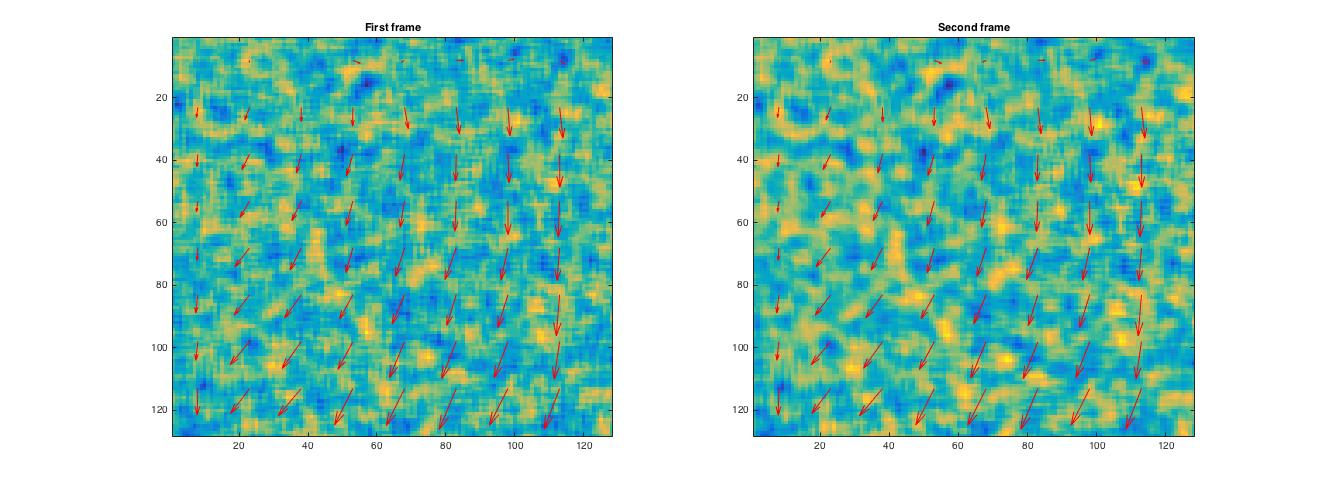
\includegraphics[width=.8\textwidth]{imgs/synth.jpg}
	\caption{Optical flow as determined by Lucas Kanade algorithm, applied to Synth images}
	\label{fig:synth_lucas}
\end{figure}


\section{Tracking}
With the previous two tools we we able to implement a simple tracking function. To do so, we first applied our implementation of Harris Corner Detector to the image at $t_1$. These were the features that were tracked along the rest of the given frames.  Then, for each pair of consecutive frames (except for the last single frame) we computed its displacement vectors which allowed us to know where the features had moved in subsequent frames. 

Since some features may move outside the camera range, we implemented a mechanism to remove them from the list of tracked points. This is important because failing to remove these points causes the tracker to try to follow them, resulting in incoherent information. Firstly, the velocity vectors would be cut in the visualizations that $quiver$ allows, but secondly and most importantly, subsequent frames would not have enough information about where those points moved afterwards and would throw null and/or unusable values.  

Once the list of feature points had been checked, we applied the Lucas-Kanade method to get the displacement vectors between each pair of subsequent frames. At this point we were able to show the image with the feature points and their corresponding vectors. Then, we updated the positions of the feature pointsaccording to their displacement and save them as the features for the next frame. 

A static visualization for our tracker is shown in Figure \ref{fig:tracker_pingpong} and \ref{fig:trackerperson}. The videos showing the tracking sequences are attached in the .zip file for the assignment delivery.

\begin{figure}[H] \centering
	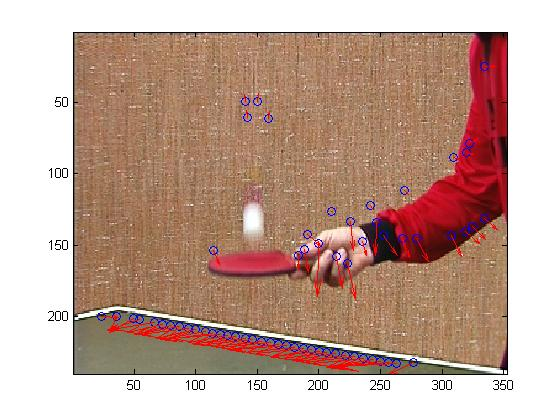
\includegraphics[width=.8\textwidth]{imgs/tracker_pingpong.jpg}
	\caption{Sample frame $t = 20$ in tracking Ping Pong images}
	\label{fig:tracker_pingpong}
\end{figure}

\begin{figure}[H] \centering
	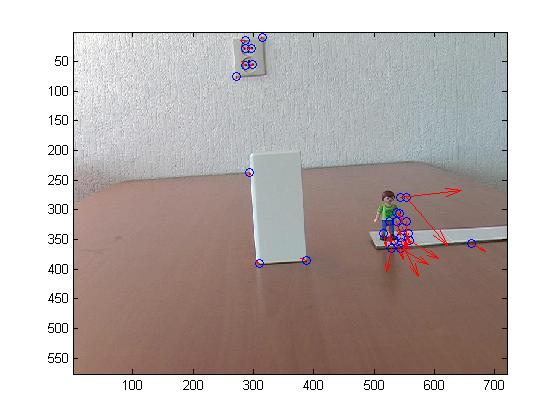
\includegraphics[width=.8\textwidth]{imgs/tracker_person.jpg}
	\caption{Sample frame $t = 20$ in tracking Ping Pong images}
	\label{fig:trackerperson}
\end{figure}

A note to keep in mind is that the returning displacement vectors have a subpixel precision. Therefore the positions need to be rounded to achieve pixel accuracy. This may be a source for noise and could lead to deterioration of the tracker performance. 

\end{document}